% key elements of prior work
% 1. eval method (sampling for large spaces)
% 2. multi-lang model, understand via boundary behavior?, different TS, examples
% 3. CM analysis, Shallow types lie
%
% SO its clear now what we mean by lying types, and the tradeoffs involved
%
% This understanding of the design space prepares for ... next question ...
%  can ask now, what is to be done
%
%

My research to date has focused on
 understanding the performance challenges for natural
 and comparing natural to other approaches.
These efforts have led up to the above thesis question.
The performance studies motivate a combination of \tdeep{} and \tshallow{}
 types, and suggest methods to empirically validate the result.
The comparison studies provide a theoretical model for defining the
 combination and understanding its formal guarantees.


\subsection{Performance Evaluation}

I began my Ph.D. studies in Fall 2014.
At this time, Typed Racket was a mature implementation of natural-style
 migratory typing.
Its type system understood compositional type tests (via occurrence typing),
 variable-arity polymorphism,
 delimited continuations,
 first-class structural classes,
 and many idioms specific to Racket programs.
Its compiler could optimize-away safety checks thanks to the static types.
It shipped with the Racket main distribution.
And it came with a base environment of useful types for many core
 libraries.

Programmers had begun using Typed Racket in various applications.
A few programmers noticed, however, that types could slow code down.
Messages appeared on the Racket mailing list documenting overheads
 of TODO and even TODO in typed code.
Invariably, these typed modules mixed with untyped code.

Prior work on Typed Racket had acknowledged that the performance of mixed-typed
 programs could be an issue.
Users experiences affirmed that performance was a crucial issue.
My first task as a Ph.D. student was thus to develop a method to assess the
 performance impact of a migratory typing system.


\subsubsection{Exhaustive Method}

In 2015, \citeN{ecoop} measured the performance impact of gradual typing on
 two object-oriented programs.
Their key insight was to begin with a fully-typed program and measure the
 running time of all gradually-typed configurations obtained by removing
 some type annotations.
By working backwards from the types, the method lets a researcher systematically
 visit the codes that a programmer may encounter as they migrate an
 application.
By measuring all configurations, the method enables general claims about
 migratory typing---which, after all, advertises the freedom to mix typed
 and untyped code.

This method for collecting data motivated a larger study~\cite{stop}.
I helped develop (and measure) 12 functional benchmark programs, ranging in
 size from 30 to 6,000 lines of code, for an evaluation of Typed
 Racket~\cite{popl}.

During the evaluation, it became clear that the data analysis was a major
 issue.
The first evaluation~\cite{ecoop} had studied two program of four modules each
 and presented the results in two powerset lattices of $2^4$ configurations.
This visualization method was impractical for programs with seven or more
 module.
The typical ``summary statistics'' of mean, median, min, and max were also a
 poor fit; although worst-case performance could be terrible
 (\figureref{fig:max-overhead}), there is no guarantee that a programmer
 will actually encounter the worst case.

To summarize our exponentially-large datasets, we formulated the notion
 of a \deliverable{D} configuration.
A mixed-typed configuration is \deliverable{D} if it runs at most $D$ times
 slower than a fully-untyped baseline configuration.
For programmers, the relevant question is what percent of all configurations
 are \deliverable{D} for a few critical values.
If a team is willing to accept a 6x slowdown due to migratory typing,
 and the percent of \deliverable{6} configurations is above 90\% on a suite
 of representative benchmarks, then they may conclude that new types are
 unlikely to break their performance goal.

Our 2016 paper~\cite{todo} plots the proportion of \deliverable{D} configurations
 for $D$ between 1x and 20x.
The results gave an extremely negative image of natural-style migratory typing;
 in half the benchmarks, fewer than 60\% of all configurations were
 \deliverable{20}.
The plots also explored whether adding types to two additional modules could
 improve performance in the best case.
Unfortunately, the extra conversions steps could not guarantee a drastic
 performance improvement.
For example, the plots in \figureref{fig:snake-popl} show the percent of
 \deliverable{D} configurations allowing 0, 1, and 2 extra conversion steps.
Even in the rightmost plot, allowing 2 angelic conversion steps, there are
 still many (~20\%) configurations that run 10 times slower than the baseline.

\begin{figure}[h]
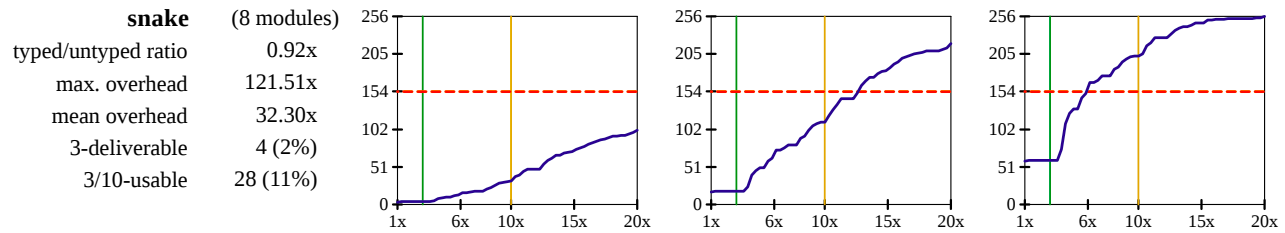
\includegraphics[width=0.96\columnwidth]{src/snake-popl.png}
\caption{Counting \deliverable{D} configurations in the \bm{snake}
         benchmark~\cite{tfgnvf-popl-2016}. The $x$-axis ranges over $D$ values;
         the vertical lines mark $D=3$ and $D=10$.
         The $y$-axis counts configurations; the dashed horizontal line marks
         $60$\% of all configs.
         The thick blue line is the number of \deliverable{x} configs.}
\label{fig:snake-popl}
\end{figure}


\subsubsection{Measuring Improvements}

The evaluation of Typed Racket inspired many efforts to improve its performance.
Sam Tobin-Hochstadt fixed issues in Typed Racket and modified it to produce
 simpler contracts for common function shapes.
Robert Bruce Findler greatly reduced the allocation costs of Racket contracts.
Others, including myself, contributed smaller patches.

All told, Typed Racket changed significantly between versions 6.2 (June 2015)
 and 6.4 (February 2016).
The evaluation method quantified the effect of these changes on
 performance with plot containing multiple \deliverable{D} curves on the same
 axis~\cite{gtnffvf-jfp-2019}.
To demonstrate, \figureref{fig:snake-jfp} presents curves for the \bm{snake}
 benchmark on Racket 6.2, 6.3, and 6.4.
The curve for version 6.4 lies above the others, meaning the percent of
 \deliverable{D} configurations is increased for every value of $D$ along
 the $x$ axis.

\begin{figure}[h]
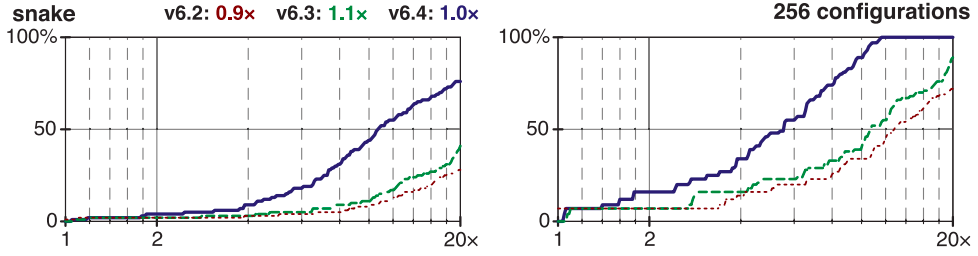
\includegraphics[width=0.8\columnwidth]{src/snake-jfp.png}
\caption{Comparing performance across three versions of Typed Racket}
\label{fig:snake-jfp}
\end{figure}

Daniel Feltey later contributed a major change to the contract system:
 collapsible higher-order contracts~\cite{fgsfs-oopsla-2018}.
Once again, the exhaustive evaluation method was one of the ways that we
 measured the impact of the new contracts.


\subsubsection{Approximate Method}

Concurrently with the improvements to Typed Racket, Zeina Migeed and I conducted
 a performance evaluation of Transient Reticulated Python.


Interesting because transient has a different strategy to enforce types.
No proxies

Challenging because Reticulated allows type annotations at a finer granularit
than TR.
For example ...

We chose to apply the method at a coarser granularity; the function
and class field.

Still too large.
Developed method to approximate the percent of \deliverable{D} configurations
by simple random sampling.

With these adaptations, evaluated Retic systematically on K benchmarks.
Found perf approx linear

Inspired a closer investigation of Retic; hence the models


\subsection{Models of Migratory Typing}


\subsubsection{Apples to Apples Comparison}

\subsubsection{Interlude: User Study}


\subsubsection{Honest vs. Lying Types}

